\documentclass{article}
\usepackage[margin=1.25in]{geometry}
\usepackage{amsmath, amssymb, setspace, enumerate, enumitem}
\usepackage{setspace}
\usepackage{graphicx}
\onehalfspacing

\begin{document}
    \begin{enumerate}
        \item \begin{enumerate}[label=(\alph*)]
            \item $k = 3$ was chosen as the optimal value for $k$, the graph is shown:\\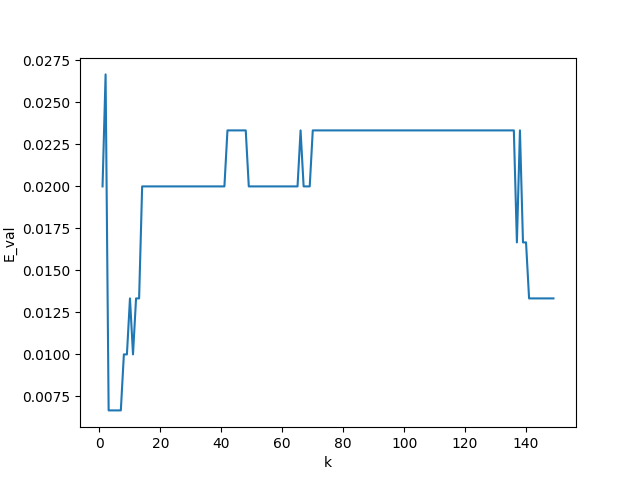
\includegraphics[scale=0.5]{images/1_a.png}
            \item For $k=3$, the decision boundary was:\\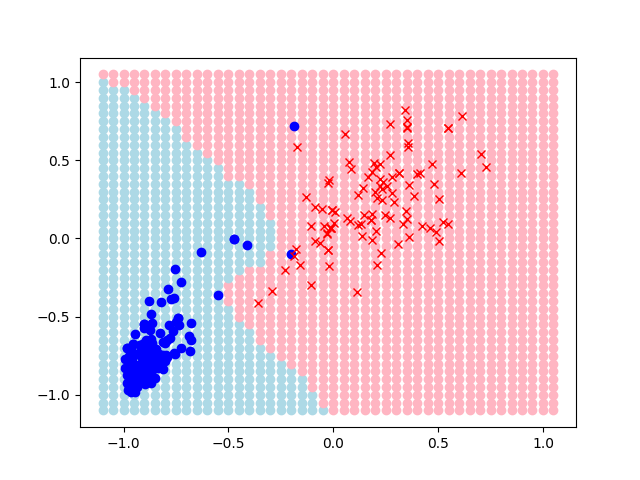
\includegraphics[scale=0.5]{images/1_b.png}\\My code uses in-sample error to choose the optimal $k$, so in sample and cross validation error were $0.0067$
            \item $0.0081$, test error was done by checking all the points in the validation set and comparing their output to what would've been the output in the training set.
        \end{enumerate}

        \item \begin{enumerate}[label=(\alph*)]
            \item The k chosen for my algorithm was $k = 2$: \\ 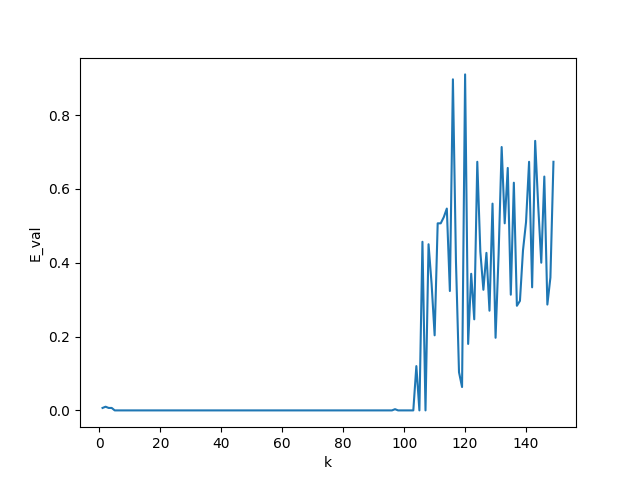
\includegraphics[scale=0.5]{images/2_a_1.png}
            \item The in sample and cross validation errors were at $0.00$, surprisingly low for my algorithm. \\ 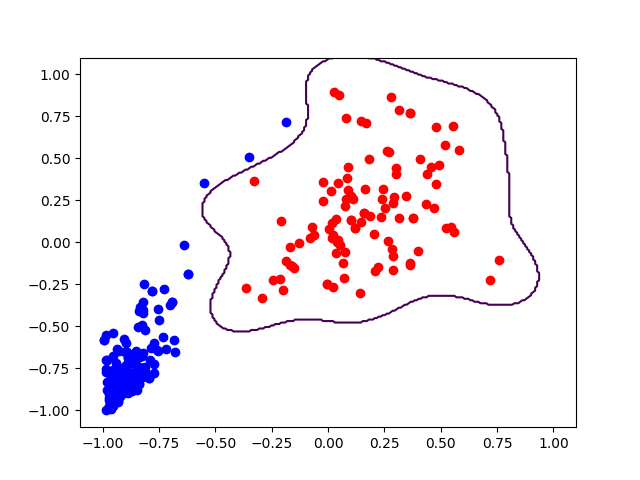
\includegraphics[scale=0.5]{images/2_b.png}\\However the data does look overfitted, which may have affected the result.
            \item When tested on the validation set, the error was high at $0.33929$, which is high and proves the overfitting problem.
        \end{enumerate}

        \item \begin{enumerate}[label=(\roman*)]
            \item linear with 8th order: 0.031
            \item k-NN: 0.0081
            \item RBF: 0.33929\\
            I believe that the way I did my RBF algorithm has small errors, after reading the book, all algorithms should relatively achieve the same performance, while the case is true for linear and k-NN, RBF does not. This makes sense since k-NN doesn't seem to use any sort of "regularizer", hence the decision boundaries for the $k_{NN}$ seem more "overfitted" even though it isn't.The linear model has a smoother curve and it seems like it bases itself better than the k-NN algorithm. \\
            We can visualize RBFs as mountains, where the nearer the neighbor is to the point, the greater weight it has on the output of the test point, RBF considers all the points, so theoretically, if RBF did work as intended, it should have the lowest $E_{out}$ out of all the algorithms since it becomes like a glorified version of the linear model.
        \end{enumerate}
    \end{enumerate}
\end{document}